% this file is called up by thesis.tex
% content in this file will be fed into the main document

\chapter{Implementation} % top level followed by section, subsection


% ----------------------- paths to graphics ------------------------

% change according to folder and file names
\ifpdf
    \graphicspath{{7/figures/PNG/}{7/figures/PDF/}{7/figures/}}
\else
    \graphicspath{{7/figures/EPS/}{7/figures/}}
\fi

\section{Framework}

In this section we describe the tools and techniques used with the OpenCSD
framework, detail modules and functionality and show the external dependencies
as well as internal relationships.

Firstly, OpenCSD consist of many external dependencies, most prominently
\textit{Storage Performance Development Kit} (SPDK) \cite{spdk} and uBPF
\cite{ubpf}. To reduce the barrier to entree and simplify ease of use OpenCSD
installs the majority of external dependencies in a local isolated build
directory. Subsequently, these dependencies are made available through an
environment file which configures variables such as \textit{PATH} and
\textit{LD\_LIBRARY\_PATH}. In addition, OpenCSD offers a QEMU installation and
accompanying qcow image to emulate a ZNS SSDs due to the limited availability of
these SSDs currently. However, the use of QEMU is entirely optional. Finally,
CMake \cite{cmake} is used to orchestrate the installation of dependencies and
binary targets. Due to limitations it is advised to rerun CMake after each make
command, this prevents unnesecarry recompilation of external
dependencies\footnotemark[9].

\footnotetext[9]{Due to limitations in the evaluation of file presence
conditions which are not reevaluated when executing the generated makefile.}

As said OpenCSD is comprised of modules using a component architecture.
Aditionally, Each module is compiled as a static or shared library to reduce
coupling. This creates an explicit nature of exchanging information between
linked libraries that allows to identify feasability problems at an early stage.
This is opposed to potentially only identifying such issues when creating a
first prototype. A trivial example of such infeasabilities would be using shared
memory mutexes to synchronize filesystem and CSx program behavior.

\subsection{Modules}

The overall modules of OpenCSD are shown in figure
\ref{figure:moduledependencies} along with any external or internal
dependencies. In addition, we briefly describe the functionality of each module.
Finally, at te end of this subsection we describe the three most prominent
modules of OpenCSd.

% Diagram with overview of different modules and their used as well as
% relationships. Also show integration of open-source technologies.

\begin{figure}
    \centering
	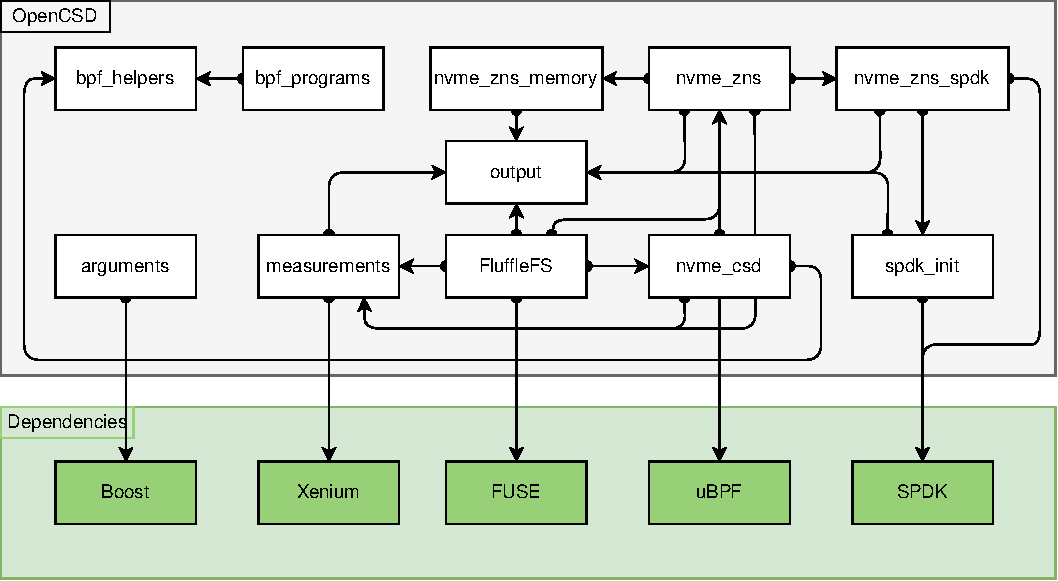
\includegraphics[width=1\textwidth]{resources/images/module-dependencies.pdf}
	\caption{Overview of all OpenCSD components and their depends-on relations}
    % \includesvg[width=0.6\columnwidth]{resources/images/module-dependencies}
    \label{figure:moduledependencies}
\end{figure}

\begin{itemize}
    \item output - Manages stdout and stderr output to the console by
    registering namespaces and providing a variety of log levels.
    \item arguments - Parses command line arguments and splits these into parts
    that can be passed to other modules in a decoupled nature. 
    \item measurements - Low overhead performance instrumentation for functions
    separated by namespaces using high performance lockless unbounded queue
    \cite{Michael1996SimpleFA}.
    \item spdk\_init - Collection of helpers to perform SPDK initialization and
    select ZNS suppporting NVMe namespace.
    \item nvme\_zns - NVMe interface to perform ZNS operations read, write and
    reset. To be used by FluffleFS for decoupled I/O operations.
    \item nvme\_zns\_memory - Memory backed implementation of nvme\_zns
    interface.
    \item nvme\_zns\_spdk - SPDK backed implementation of nvme\_zns interface
    \item nvme\_csd - Simulated extension to the PCIe NVMe protocol that allows
    to perform CSx operations. Execution of kernels is handled through uBPF.
    Utilizes instance of nvme\_zns to perform actual I/O operations performed by
    kernel.
    \item bpf\_helpers - Collection of headers that define the eBPF
    \textit{Application Binary Interface} (ABI) supported for CSx
    \textit{kernel}s. ABI to be implemented by device vendor or in this
    case nvme\_csd for simulation. The ABI is filesystem agnostic.
    \item bpf\_programs - Collection of eBPF programs linked at runtime for
    previous ZCSD \cite{lukken2021zcsd} prototype.
    \item FluffleFs - FUSE LFS supporting in-memory snapshots to achieve
    multi-user tenancy with concurrent regular and offloaded filesystem access.
    Utilizes, nvme\_zns and nvme\_csd to achieve functionality.
\end{itemize}

Out of these comoponents nvme\_csd, bpf\_helpers and FluffleFS are the most
essential. They simulate the required changes that would be required to
realize the architecture as proposed in our simulation framework. The details of
such a practical architecture will be described in details later.

In short nvme\_csd contains functions that should be made part of a new NVMe
command set and namespace \cite{nvme-command} similar to how ZNS was introduced.
The functions are overlie simplified so there is no use of the actual command
layout as well as lack of queue submissions and completion commands. We feel
the concepts of implementing these are well understood and would not contribute
to the scientific value of this work while introducing substantial additional
complexity.

bpf\_helpers contains the ABI exposed to the eBPF kernels. An ABI is different
from an API in that the functions it defines can not be found in segments of
code, either included statically or through a shared library. Instead it uses
an ISA specific instruction that can be called with a set of arguments, the
arguments matching the function signature. Alternatively, should the ISA not
have a specific \textit{call} instruction, interrupt requests can be used to
achieve the same functionality. Upon calling the control flow is returned to
the operating system or in our case uBPF where the functions behavior is
implemented. The result is that an ABI allows to define functionality with
vendor agnostic implementations, similar to POSIX for operating systems. It
should be noted that ISAs typically have a hard limit on the number of arguments
that can be supported, in the case of eBPF this is five arguments.

Lastly, is FluffleFS which is described in the next separate section in detail.

\section{Filesystem}

% Two write pointers, one for RANDOM ZONE and one for LOG ZONE. Use of ZNS is
% optional but allows for lower write-amplification and more explicit garbage
% collection

\subsection{Concurrency}

\section{Offloading}

% Filesystem extended attributes, PID + INODE

% ---------------------------------------------------------------------------
% ----------------------- end of thesis sub-document ------------------------
% ---------------------------------------------------------------------------